% \documentclass{beamer}
% \usepackage{tikz}
\usetikzlibrary{arrows, positioning}

% \usetikzlibrary{positioning}
% \title{Simple Traffic Flow}
% \date{}



% Equations
\begin{frame}{Equations}
\centering
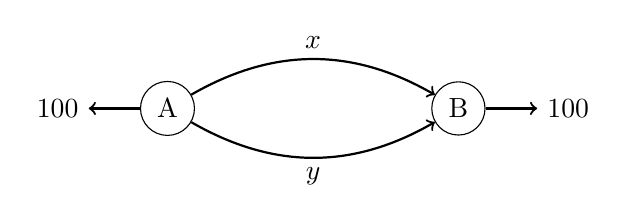
\begin{tikzpicture}[node distance=3cm]
  \node[circle,draw] (A) {A};
  \node[circle,draw, right=of A] (B) {B};
  \draw[->, thick, bend left] (A) to node[above] {\(x\)} (B);
  \draw[->, thick, bend right] (A) to node[below] {\(y\)} (B);
  \draw[->, thick] (A) -- ++(-1,0) node[left]{100};
  \draw[->, thick] (B) -- ++(1,0) node[right]{100};
\end{tikzpicture}
\[
x+y=100,\quad x-y=20.
\]
\end{frame}

% Method 1: Systems of Equations
\begin{frame}{Solution: Equations}
\[
(x+y)+(x-y)=120\quad\Rightarrow\quad 2x=120,\; x=60.
\]
\[
y=100-60=40.
\]
\end{frame}

% Method 2: Linear Algebra (Row Reduction)
\begin{frame}{Solution: Linear Algebra}
\[
\begin{bmatrix} 1 & 1\\ 1 & -1 \end{bmatrix}
\begin{bmatrix} x\\ y \end{bmatrix}=
\begin{bmatrix} 100\\ 20 \end{bmatrix}.
\]
Augmented matrix:
\[
\left[\begin{array}{cc|c}
1 & 1 & 100\\[1mm]
1 & -1 & 20
\end{array}\right]
\]
Subtract \(R_1\) from \(R_2\):
\[
\left[\begin{array}{cc|c}
1 & 1 & 100\\[1mm]
0 & -2 & -80
\end{array}\right]
\quad\Rightarrow\quad y=40,\; x=60.
\]
\end{frame}

\end{document}
